\section{Results}
\begin{figure}[ht]
	\centering
	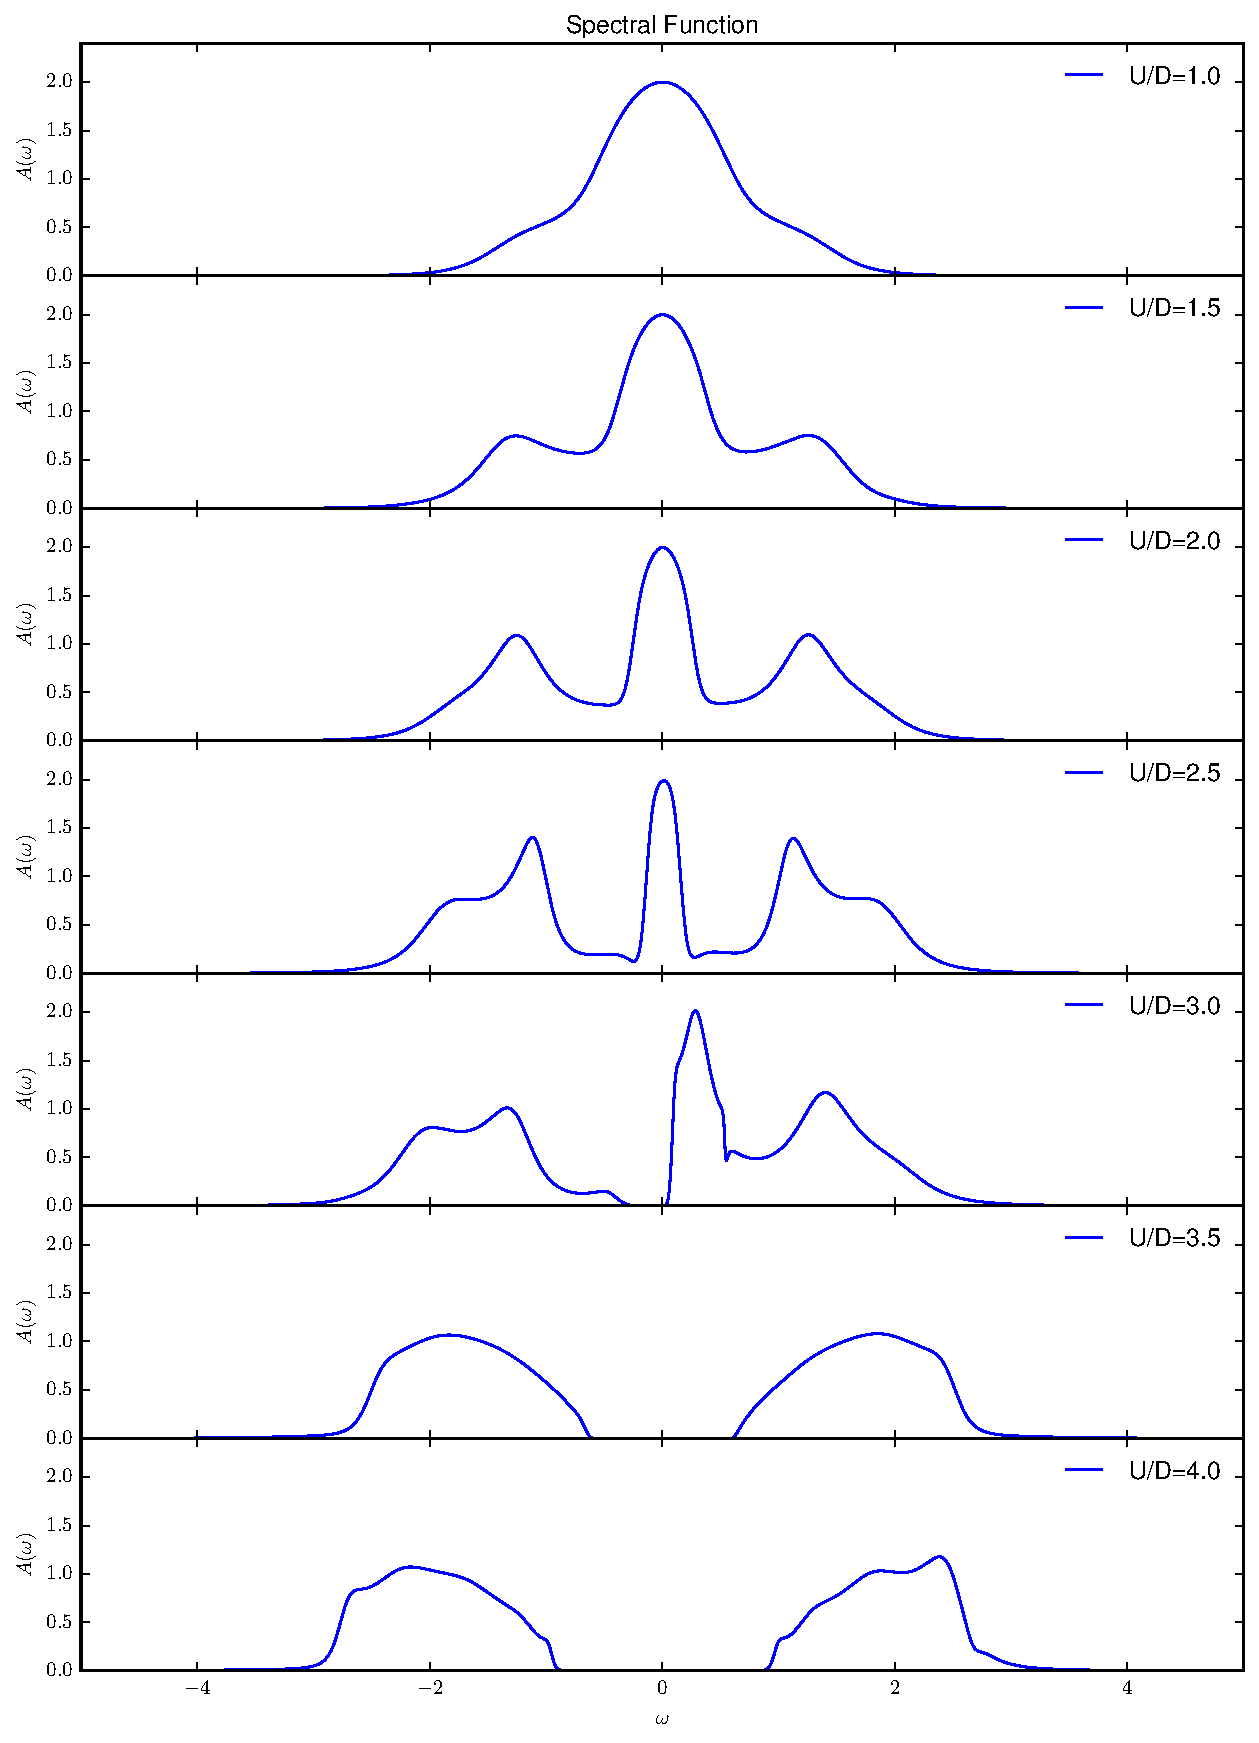
\includegraphics[width=0.5\textwidth ]{Mott_transition}
	\caption{Spectral function after analytic continuation. For low interaction parameter $U$ there are single particle excitation??? at zero frequency, therefore the metalic phase. With increasing interaction parameter the spectral function develops a gap at zeros freqency, hence no excitation, ie the insulator phase.}
	\label{fig:spectralf}
\end{figure}
As final result of our simulation, we obtained the plots of the Spectral~Function for increasing values of the interaction strenght $U$ (see \figref{fig:spectralf}).

It can be cleary seen that with increasing interaction we observe a phase transition (in our case between $3<U<4$) from a conductor to a Mott insulator, which is exactly what we exspected to find. 

This deduction from the values of the spectral function at varying $U$ becomes clear if we recall the meaning of this function.  
In particular, for the Fermionic case, the single-particle Spectral~Function, $\mathscr{A(\bold{k},\omega)}$, can be expressed in the Lehmann representation: 

\begin{equation}\label{S.P.}
\mathscr{A}_\sigma(\bold{k},\omega) = \frac{1}{\mathcal{Z}}\sum_{n,m}|\braket{m|c_\bold{\sigma,k}^\dagger|n}|^2 (e^{-\beta E_n} + e^{-\beta E_m})\delta(\omega+(E_n-E_m)))
\end{equation}
where the $\ket{n}$'s are the Hamiltonian eigenstates and the $E_n$'s are the corresponding energies. 
Starting from this expression it is also possible to show that the following sum rule holds:

\begin{equation}
\int_{-\infty}^\infty \mathscr{A}_\sigma(\bold{k},\omega)d\omega = 1
\end{equation}
If one notice, moreover, that $\mathscr{A}_\sigma \geq 0$, it is, then, possible to interpret
it as a probability density. In particular, usually, this is interpreted as the probability of having a fermion with energy between $\omega$ and $\omega + d\omega$.

One could also consider the single-particle density of states, $D(\omega)$, which is given by:

\begin{equation}\label{D.o.S.}
D(\omega) = \frac{1}{V}\sum_{\bold{k},\sigma} \mathscr{A}_\sigma(\bold{k},\omega)
\end{equation}
at the light of this expression and of equation \eqref{S.P.}, it is clear, then, that no gaps in the Spectral Function (as in our plots for low values of $U$) means that we can produce exitations with any energy, leading to a conductor behaviour. Whereas, if a gap is present (as in the last plot of Refenrence ??) it means that no exitations can be produced with thise energy, so that the material will behave as an insulator.


\clearpage
